\documentclass[12pt]{aghdpl}
\graphicspath{ {img/} }
\usepackage{svg}
\usepackage{pgfplots}
% \documentclass[en,11pt]{aghdpl}  % praca w języku angielskim

% Lista wszystkich języków stanowiących języki pozycji bibliograficznych użytych w pracy.
% (Zgodnie z zasadami tworzenia bibliografii każda pozycja powinna zostać utworzona zgodnie z zasadami języka, w którym dana publikacja została napisana.)
\usepackage[english,polish]{babel}

% Użyj polskiego łamania wyrazów (zamiast domyślnego angielskiego).
\usepackage{polski}

\usepackage[utf8]{inputenc}

% dodatkowe pakiety

\usepackage{mathtools}
\usepackage{amsfonts}
\usepackage{amsmath}
\usepackage{amsthm}

% --- < bibliografia > ---

\usepackage[
style=numeric,
sorting=none,
%
% Zastosuj styl wpisu bibliograficznego właściwy językowi publikacji.
language=autobib,
autolang=other,
% Zapisuj datę dostępu do strony WWW w formacie RRRR-MM-DD.
urldate=edtf,
% Nie dodawaj numerów stron, na których występuje cytowanie.
backref=false,
% Podawaj ISBN.
isbn=true,
% Nie podawaj URL-i, o ile nie jest to konieczne.
url=false,
%
% Ustawienia związane z polskimi normami dla bibliografii.
maxbibnames=3,
% Jeżeli używamy BibTeXa:
backend=bibtex
]{biblatex}

\usepackage{csquotes}
% Ponieważ `csquotes` nie posiada polskiego stylu, można skorzystać z mocno zbliżonego stylu chorwackiego.
\DeclareQuoteAlias{croatian}{polish}

\addbibresource{bibliografia.bib}

% Nie wyświetlaj wybranych pól.
%\AtEveryBibitem{\clearfield{note}}


% ------------------------
% --- < listingi > ---

% Użyj czcionki kroju Courier.
\usepackage{courier}

\usepackage{listings}
\lstloadlanguages{TeX}

\lstset{
	literate={ą}{{\k{a}}}1
           {ć}{{\'c}}1
           {ę}{{\k{e}}}1
           {ó}{{\'o}}1
           {ń}{{\'n}}1
           {ł}{{\l{}}}1
           {ś}{{\'s}}1
           {ź}{{\'z}}1
           {ż}{{\.z}}1
           {Ą}{{\k{A}}}1
           {Ć}{{\'C}}1
           {Ę}{{\k{E}}}1
           {Ó}{{\'O}}1
           {Ń}{{\'N}}1
           {Ł}{{\L{}}}1
           {Ś}{{\'S}}1
           {Ź}{{\'Z}}1
           {Ż}{{\.Z}}1,
	basicstyle=\footnotesize\ttfamily,
}

% ------------------------

\AtBeginDocument{
	\renewcommand{\tablename}{Tabela}
	\renewcommand{\figurename}{Rys.}
}

% ------------------------
% --- < tabele > ---

\usepackage{array}
\usepackage{tabularx}
\usepackage{multirow}
\usepackage{booktabs}
\usepackage{makecell}
\usepackage[flushleft]{threeparttable}

% defines the X column to use m (\parbox[c]) instead of p (`parbox[t]`)
\newcolumntype{C}[1]{>{\hsize=#1\hsize\centering\arraybackslash}X}


%---------------------------------------------------------------------------

\author{Michał Gandor}
\shortauthor{M. Gandor}

%\titlePL{Przygotowanie bardzo długiej i pasjonującej pracy dyplomowej w~systemie~\LaTeX}
%\titleEN{Preparation of a very long and fascinating bachelor or master thesis in \LaTeX}

\titlePL{Symulacja dynamiki pieszych z wykorzystaniem modelu Social Force.}
\titleEN{Simulation of pedestrian dynamics using Social Force Model.  }

\shorttitlePL{Symulacja dynamiki pieszych z wykorzystaniem modelu Social Force.}
\shorttitleEN{Simulation of pedestrian dynamics using Social Force Model.  }

\thesistype{Praca dyplomowa inżynierska}
%\thesistype{Master of Science Thesis}

\supervisor{dr hab. inż. Jarosław Wąs}
%\supervisor{Marcin Szpyrka PhD, DSc}

\degreeprogramme{Informatyka}
%\degreeprogramme{Computer Science}

\date{2017}

\department{Katedra Informatyki Stosowanej}
%\department{Department of Applied Computer Science}

\faculty{Wydział Elektrotechniki, Automatyki,\protect\\[-1mm] Informatyki i Inżynierii Biomedycznej}
%\faculty{Faculty of Electrical Engineering, Automatics, Computer Science and Biomedical Engineering}

\acknowledgements{Serdecznie dziękuję \dots tu ciąg dalszych podziękowań np. dla promotora, żony, sąsiada itp.}


\setlength{\cftsecnumwidth}{10mm}

%---------------------------------------------------------------------------
\setcounter{secnumdepth}{4}
\brokenpenalty=10000\relax

\begin{document}

\titlepages

% Ponowne zdefiniowanie stylu `plain`, aby usunąć numer strony z pierwszej strony spisu treści i poszczególnych rozdziałów.
\fancypagestyle{plain}
{
	% Usuń nagłówek i stopkę
	\fancyhf{}
	% Usuń linie.
	\renewcommand{\headrulewidth}{0pt}
	\renewcommand{\footrulewidth}{0pt}
}

\setcounter{tocdepth}{2}
\tableofcontents
\clearpage

\chapter{Wprowadzenie}
\label{cha:wprowadzenie}

Zachowanie tłumu badane jest od przeszło trzech dekad. Na samym początku badania były traktowane w ramach ciekawostki. Wraz z nowatorskimi pracami Helbinga .... . W ostatnich latach zagadnienie to zyskuje coraz większe znaczenie. Jesteśmy obecnie świadkami rozrostu miast, budowy kompleksów sportowych czy galerii handlowych. Wszystkie te miejsca są nieodłącznie związane z tłumami przewijających się przez nie osób. W związku z rosnącą gęstością zaludnienia oraz wzrostem zagoreń takich jak terroryzm [jakis przypis] tworzenie symulacji ewakuacji nabrało większego znaczenia. Dzięki zasymulowaniu zachowania tłumu możenmy łatwiej utworzyć schematy opuszczenia bynków podczaz zagorżenia minimaliusjąc szkody oraz ofiary. Symulacje pozwalają także na lepsze rozładowanie ruchu drogowego w miastach o roznącej ilości zaludnienia.

Symulacje mogą mieć wielorakie zastosowanie, począwszy od ewakucaji ludności poprzez zachowania w centrach handlowych kończąc na ruchu drogowym. Na przejściach dla pieszych w Japonii ginie 30\% osób uczestniczących w wypadkach drogowych \cite{AMSFMfPBSaSC}, a w Niemczech odsetek ten wynosi 15\% \ [German instigute for econeomic research 2010]. Zgodnie z danymi organizacjie Fire Administration w Stanach Zjednoczonych \cite{Asfemwle} w roku 2007 3430 osób zmarło w pożarach oraz blisko 18 tysięcy zostało ranych.

%---------------------------------------------------------------------------

\section{Cele pracy}
\label{sec:celePracy}

Celem poniższej pracy jest zapoznanie studentów z systemem \LaTeX~w zakresie umożliwiającym im samodzielne, profesjonalne złożenie pracy dyplomowej w systemie \LaTeX.

%---------------------------------------------------------------------------

\section{Zawartość pracy}
\label{sec:zawartoscPracy}

W rodziale~\ref{cha:pierwszyDokument} przedstawiono podstawowe informacje dotyczące struktury dokumentów w \LaTeX u. Alvis~\cite{Alvis2011} jest językiem 



















\chapter{Wykaz ważniejszych oznaczeń}
\label{sec:wykazOznaczen}

SFM - Social Force Model
A* - algorytm A Star
POI - points of intrests
[do dopisania]

















\chapter{Wprowadzenie teoretyczne}
\label{cha:wprowadzenieTeoretyczne}

Dziedziny nauki badające ruch pieszych to nie tylko informatyka. Na powstanie modeli miały także wpływ prace uczonych z takich dziedzin jak psychologia, socjologia czy architektura. Problem zachowania tłumu jest skomplikowany i dopiero połączenie tych wszystkich dziedzin dało początek realnemu odzwierciedleniu na ekranie komputera. \\
Z pozoru zachowanie pieszych może wydawać się chaotyczne oraz trudne do przewidzenia. Bazując jednak na badaniach i obserwacjach takie zachowania mają miejsce tylko w skrajnych przypadkach. W codziennym życiu okazuje się, że model do opisu zachowania tłumu może być w dość prosty sposób opisany, głównie dzięki prawdopodobieństwom jakie mogą zostać nakreślone w dużych populacjach ludzi. Człowiek ma tendencję do podejmowania decyzji na bazie posiadanej już wcześniej, wypracowanej wiedzy na temat otaczającego go środowiska. Oznacza to, że reakcje na innych pieszych oraz przeszkody mogą być w łatwy sposób przewidziane. Analogią do takiego zachowania mogą być przykładowo reakcje profesjonalnego kierowcy wyścigowego, który reaguje na sytuacje drogowe niemal automatycznie.

Oczywiście nie jest to prawdą w każdej sytuacji. Przykładowo dzieci oraz turyści wykazują inny sposób poruszania się za względu na to, że zazwyczaj znajdują się w nowym miejscu i nie mają wypracowanej strategii poruszania się. Jednakże dla potrzeb symulacji nie potrzeba dokładnych informacji o każdym z pieszych. W zupełności wystarcza statystyczna wartość konkretnych zachowań

W tym rozdziale zostają przedstawione podstawowe dostępne obecnie modele. Każdy z modeli ma swoje zalety oraz wady, wpływają na to cechy takie jak złożoność obliczeniowa, złożoność implementacji oraz oczywiście cechy otrzymanych rezultatów.

\section{Klasyfikacja modeli symulacji ruchu pieszych}
\label{sec:klasyfikacja}

\subsection{Modele mikroskopowe oraz makrospokope}

Modele makroskopowe pokazują w głównej mierze dynamikę gęstości oraz prędkości całego tłumu. W tym celu używane są istniejące już modele fizyczne takie jak dynamika płynów, które zostają odpowiednio dostosowane do potrzeb symulacji. Przykładem może być hydrodynamiczny model Paulusa opierający się na równaniach przepływu \cite{ArchitekturaModelowania}. Modele te nie biorą pod uwagę indywidualnych zachowań jednostki.\\

Podejście makrospokowe ze względu na odzwierciedlanie całej populacji sprawdza się w praktyce tylko w wąskim wachlarzu zastosowań.
 
Jako zaletę podejścia makroskopowego możemy z pewnością wskazać mniejszą ilość obliczeń potrzebną do uzyskania porządanego efektu.

Modele mikrospokowe, w przeciwieństwie do wspomnianych wyżej modeli makroskopowych, biorą one pod uwagę zachowanie konkretnej jednostki. Badane są interakcje pomiędzy pieszymi oraz ich iteracje z przeszkodami oraz otaczającą rzeczywistością. Modele te pozwalają na uzyskanie efekty bardziej odpowiadającego realnemu zachowaniu tłumu. Jednakże wraz ze wzrostem odwzorowania detali wzrasta również złożoność systemu oraz zwiększa się złożoność obliczeń co skutkuje toeretycznie gorszą wydajnością, jednak przy dostępnej obecnie mocy obliczeniowej nawet standardowych komputerów nie gra to aż takiej roli.

\subsection{Modele ciągłe i dyskretne}

W modelach mikroskopowych możemy wyodrębinić dwie podgrupy: modele ciągłe oraz dyskretne. Modele dyskretne cechują się zmianą paramatrów stanu w konkretnych interwałąch czasowych, przyjmują okręślone wartości dla określonych argumantów i tylko dla nich. W modelach ciągłych stan ulega zmienie przez cały czas działania, może przyjmować dowonlą wartość z całego przedziału. Modele ciągłe reprezentują oczywiście dane w sposób bardziej realistyczny, jednakże zwiększają czas obliczeń \\

Jednym z przykładów na model dyskretny może być automat komórkowy. Uniwersalność automatów komórkowych \textit{Cellular Automata} spowodowała, iż znajdują zastosowanie także w dziedzinie symulacji ruchu pieszych. Automat komórkowy jest modelem matematycznym, który specyfikuje siatka komórek, zbiór stanów jakie mogą one przyjmować, oraz reguły określające stan komórki w chwili $t + 1$. Stan danej komórki zależny jest od stanu komórek z nią sąsiadujących w chwili $t$. \\

Dla stworzenia modeli mikroskopowych używano z początku niehomogenicznych automatów komórkowych. Wraz z rozwojem symulacji na automatach komórkowych można było dostrzec duże zmiany bazowym modelu. Powstające symulacje zaczęły zostać klasyfikowane jako \textbf{sytemy agentowe}.

Niestety jednorodność tej metody uniemożliwia modelowanie bardziej skomplikowanych procesów\cite{FormalizacjaAutomatów}.

%---------------------------------------------------------------------------



















\chapter{Wyznaczenie ścieżki}
\label{cha:wyznaczenieSciezki}

Wyznaczenie najkrótszych ścieżek jest jednym z podstawowych problemów w teorii grafów. Algorytmy wyszukiwania ścieżek mają wielorakie zastosowanie, począwszy od wyznaczenia najkrótszych tras na mapie, poprzez przesyłanie wiadomości przez sieć routerów, kończąc na wyznaczaniu połączeń lotniczych o najmniejszym koszcie. Wynikiem działania algorytmów wyznaczania ścieżek jest uporządkowany zbiór wierzchołków, którymi należy kolejno podążać, aby dotrzeć do wyznaczonego wcześniej celu. Podczas symulacji algorytm wykorzystywany jest w pierwszym kroku. Przed właściwym uruchomieniem symulacji zostają wyznaczone najkrótsze ścieżki prowadzące każdego z pieszych do celu, które są później podstawą do dla działania SFM.

Algorytmów wyszukiwania ścieżek jest bardzo wiele, najważniejsze z nich to:

\begin{itemize}
\item Algorytm Dijkstry - przykład algorytmu zachłannego. Jeden z najbardziej rozpowszechnionych algorytmów w dziedzinie przeszukiwania ścieżek. Jego złożoność obliczeniowa rośnie w miarę wzrostu punktów węzłowych,
\item Algorytm A* - jest to rozszerzona wersja algorytmu Dijkstry. Dzięki zastosowaniu heurystyki skraca się czas obliczeń,
\item Algorytm Bellmana-Forda - ma zastosowanie, kiedy niektóre krawędzie w grafie mają ujemne wagi
\item Algorytm Floyda-Warshalla - pozwala na odnalezienie najkrótszych ścieżek pomiędzy wszystkimi parami wierzchołków w grafie,
\item Przeszukiwanie wszerz BFS - najprostszy z algorytmów, nie uwzględnia wag ścieżek,
\item Przeszukiwanie wgłąb DFS - podobny do algorytmu BFS, wymaga mniej zasobów oraz jest szybszy.
\end{itemize}

W symulacji przeprowadzonej na potrzeby tej pracy został zastosowany Algorytm A*. Gwarantuje on zawsze znalezienie optymalnej ścieżki, jeśli tylko istnieje. Jego użycie nie wymaga także szczególnie skomplikowanych obliczeń. Algorytm A* jest znacznie szybszy w porównaniu do Algorytmu Dijkstry. Nie tylko czas wyszukiwania ścieżki jest krótszy, ale również ilość odwiedzonych elementów na mapie jest mniejsza, co skutkuję mniejszą złożonością pamięciową. W przeprowadzonych przez autora porównaniach, Algorytm A* pozwala na średnio $16 sekund$ szybsze wyszukanie ścieżki odwiedzając średnio $1710$ węzłów mniej niż Algorytm Dijkstry. Działanie algorytmów przedstawiają rysunki \ref{fig:djikstra} oraz \ref{fig:astar}. Kolor fioletowy oznacza odwiedzone węzły, zielony węzeł początkowy, a czerwony końcowy. Kolorem żółtym oznaczona została wyznaczona ścieżka.

\begin{figure}
\label{fig:djikstra}
\centering
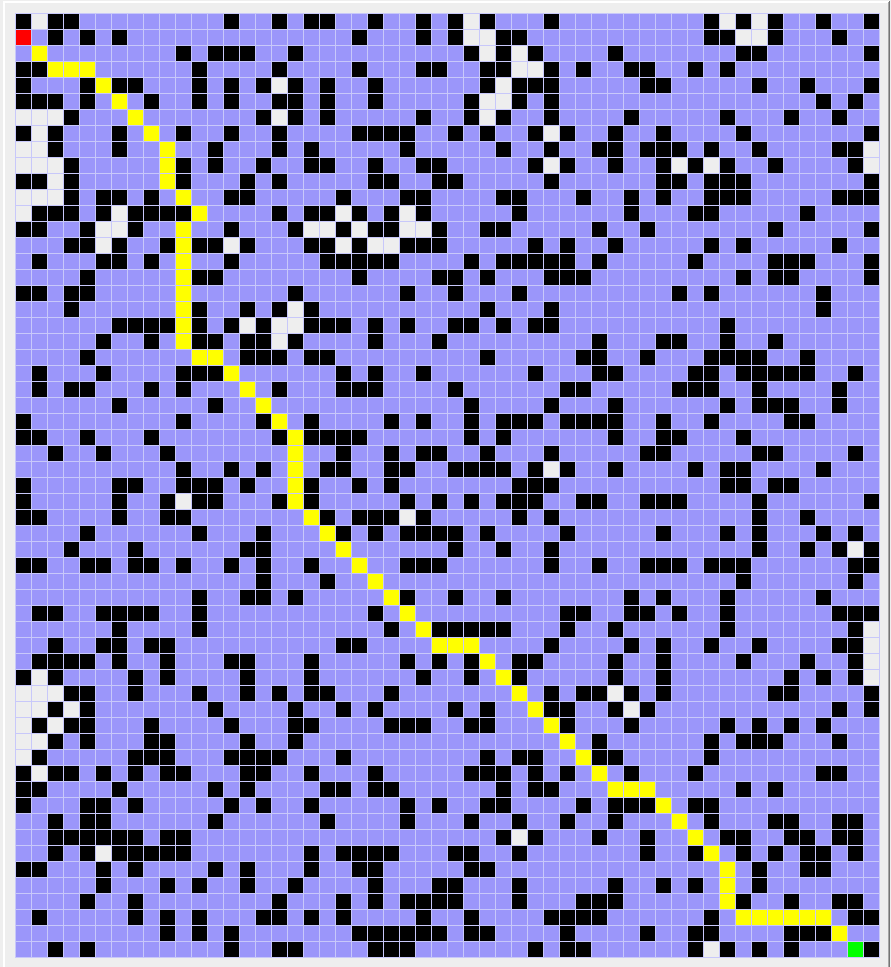
\includegraphics[width=0.5\textwidth]{djikstra.png}
\caption{Wizualizacja algorytmu Dijkstry \cite{searchpathsimplementations}}
\end{figure}

\begin{figure}
\label{fig:astar}
\centering
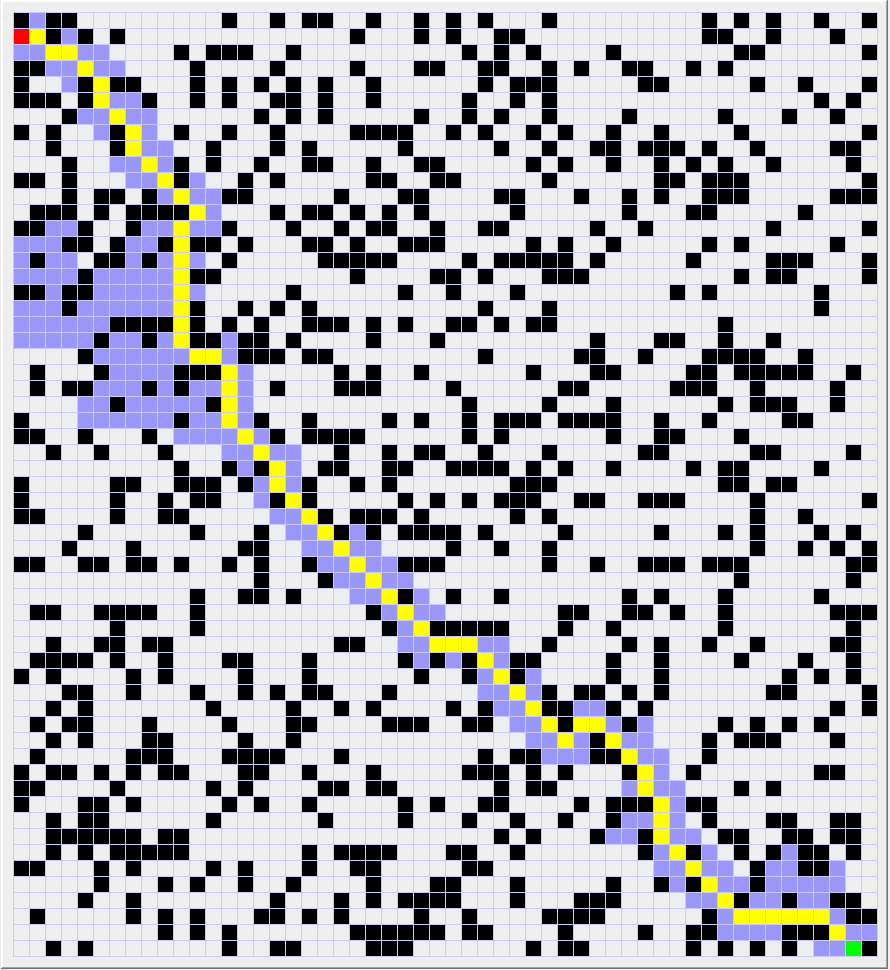
\includegraphics[width=0.5\textwidth]{astar.png}
\caption{Wizualizacja algorytmu A*, \cite{searchpathsimplementations}}
\end{figure}
\chapter{Opis modelu Social Force}
\label{cha:OpisSocialForce}

Model Social Force \cite{SforceModelForPedDyn}, bezsprzecznie najważniejszy z obecnie dostępnych, jest mikrospokowym modelem ciągłym. Zakłada on, że piesi w ruchu mogą zostać w prosty sposób opisani za pomocą sił. Siły te pochodzą nie tylko z oddziaływań konkretnego pieszego na otoczenie, ale także z otoczenia na danego pieszego. Wartość, zwrot oraz kierunek siły finalnej jest składową wszystkich sił działających na danego pieszego. Piesi w modelu reprezentowani są za pomocą cząstek, które dążą do celu w konkretnych kierunkach oraz są pod działaniem wspomnianych sił. Dotychczasowe symulacje komputerowe pokazują, że Model Social Force, pomimo swojej prostoty bardzo realistycznie oddaje rzeczywiste zachowanie tłumu.

\begin{figure}
\centering
\includegraphics[width=0.5\textwidth]{process.eps}
\caption{Schemat podejmowania decyzji przez pieszego, opracowanie własne na bazie \cite{GuideCrowdDynViaModifiedSocialForceModel}}
\end{figure}

Nie bez znaczenia jest także łatwość uzyskania parametrów oraz wartości potrzebnych do symulacji. Wartości takie jak predkość $\vec{v_{\alpha}}$ czy położenie $\vec{r_{\alpha}}$ danego pieszego $\alpha$ są łatwe do obliczenia, ale także do skalibrowania z danami empirycznymi.

Pierwsze symulacje korzystające z modelu SF były skupione głównie na ewakuacjach budynków. W tego typu sytuacjach celem pieszego jest dojście do wyjścia w możliwie najkrótszym czasie. Obecnie istnieje mnogość wariantów modelu, które pozwalają na zamodelowanie większej ilości zachowań. Obecne modyfikacje przewidują przykładowo unikanie "spychania" innych uczestników ruchu poprzez pieszych poruszających się z większą prędkością \cite{6}.

Istnieje bardzo wiele różnych modyfikacji modelu Social Forca. Wykorzystany w pracy model \cite{GuideCrowdDynViaModifiedSocialForceModel} bazuje na oryginalnym modelu Helbinga \cite{SforceModelForPedDyn} zakłada, że na pieszego działają trzy siły. Desired force $\vec{f_{i}^{0}}$, siła interakcji pomiędzy pieszymi $i$ oraz $j$, $\vec{f_{ij}}$ oraz siła interakcji pomiędzy pieszym $i$, a przeszkodami, $\vec{f_{iw}}$

Siła działająca na każdego z pieszych definiuje się jako:

\begin{equation}
m_{i} \frac{d\vec{v_{i}}(t)}{dt} = \vec{f_{i}^{0}} + \sum_{j(\neq i)} \vec{f_{ij}} + \sum _{w} \vec{f_{iw}}
\end{equation}

gdzie
\begin{eqwhere}[2cm]
	\item[$m_{i}$] masa pieszego $i$
	\item[$\vec{v}_{i}(t)$] aktualna prędkość
\end{eqwhere}

\section{Desired force}
\label{sec:desiredForce}

Bazując na obserwacjach można wywnioskować, że piesi wykazują niechęć do zmiany prędkości oraz kierunku swojej drogi. Zazwyczaj wybierana jest droga, którą można podążać prosto przez jak najdłuższy okres czasu, nawet jeśli drogi alternatywne są takiej samej długości, a droga wybrana przez pieszego jest mocno zatłoczona. Kierunek ruchu obliczany jest na podstawie wzoru:

\begin{equation}
\vec{e}_{\alpha}(t) = \frac{\vec{r}_{\alpha}^{k} - \vec{r}_{\alpha}(t)}{\parallel \vec{r}_{\alpha}^{k} - \vec{r}_{\alpha}(t) \parallel}
\end{equation}

gdzie
\begin{eqwhere}[2cm]
	\item[$e_{\alpha}(t)$] aktualna pozycja pieszego $\alpha$ w czasie $t$
	\item[$\vec{r}_{\alpha}^{k}$] najbliższy punkt na ścieżce do celu
\end{eqwhere}

\begin{figure}
\centering
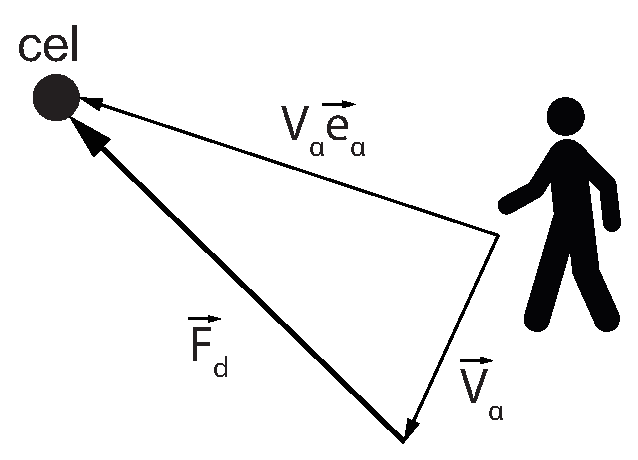
\includegraphics[width=0.5\textwidth]{desiredforce2.eps}
\caption{Schemat siły \textit{desired force} , opracowanie własne na bazie \cite{AMSFMfPBSaSC}}
\end{figure}

\begin{figure}
\centering
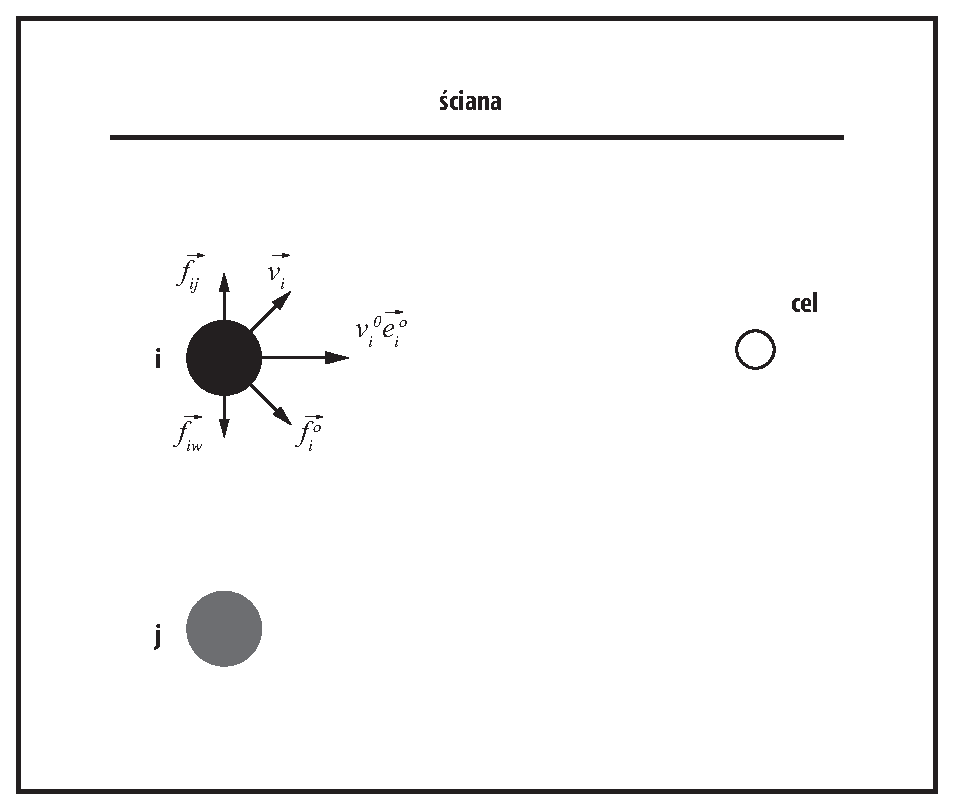
\includegraphics[width=0.5\textwidth]{desiredforce.eps}
\caption{Diagram modelu Social Force, opracowanie własne na bazie \cite{GuideCrowdDynViaModifiedSocialForceModel}}
\end{figure}

W przypadku kiedy ruch pieszego odbywa się bez przeszkód porusza się on w kierunku pozycji celu, z preferowaną przez siebie prędkością, $\vec{v_{i}^{0}}$. Z powodu działania na pieszego sił~z otoczenia, obserwuje się dążenie pieszego do osiągnięcia preferowanej przez siebie prędkości w czasie relaksacji $\tau$.

\begin{equation}
\vec{f}_{i}^{0} = m_{i} \frac{v_{i}^{0}(t) \vec{e_{i}^{0}} - \vec{v_{i}}(t)}{\tau}
\end{equation}

gdzie
\begin{eqwhere}[2cm]
	\item[$\vec{v_{i}^{0}}$] wartość domyślnej prędkości pieszego
	\item[$\vec{e_{i}^{0}}$] kierunek ruchu jaki pieszy chce osiągnąć
	\item[$\tau$] czas relaksacji
\end{eqwhere}
	
Jest to tzw. \textit{desired speed} [wyjaśnić], odzwierciedla ona dążenie danego pieszego $i$ do osiągnięcia preferowanej prędkości.

Domyślna prędkość pieszego przyjmuje zazwyczaj wartość około $1.34 \frac{m}{s^{2}}$ z odchyleniem standardowym $0.26 \frac{m}{s^{2}}$ \cite{HeBuAjTw}

\section{Interakcja pomiędzy pieszymi}
\label{sec:interactionBetweenPedestrians}

Naturalnym jest, że kiedy zbliżamy się do innych uczestników ruchu czujemy się niekomfortowo. Zakłada się, że każdy z pieszych, który jest w konflikcie z innym uczestnikiem ruchu generuje wokół siebie eliptyczne pole siły, które działa na drugiego z pieszych. Aby uniknąć wypadków utrzymują dystans pomiędzy innymi uczestnikami ruchu oraz przeszkodami. Dystans ten zmniejsza się w przypadku kiedy pieszy śpieszy się oraz kiedy wzrasta gęstość tłumu. Gęstość tłumu zwiększa się w szczególności kiedy piesi znajdują się w okolicy miejsc wywierających zainteresowanie oraz w wąskich przejściach. Siła interakcji pomiędzy pieszymi $i$ oraz $j$, $\vec{f_{ij}}$ definiowana jest jako suma dwóch sił, socjologiczno-psychologicznej oraz fizycznej. Piesi mogą także formować grupy, których zachowanie można później sprowadzić do opisu pojedynczego agenta \cite{HeBuAjTw}

\begin{equation}
\vec{f_{ij}} = \vec{f}_{ij}^{s} + \vec{f}_{ij}^{p}
\end{equation}
Pierwsza z nich $\vec{f_{ij}^{s}}$ związana jest z naturalnym ludzkim odruchem utrzymywania dystansu od drugiego człowieka. Przyjmuje ona wartość maksymalną, gdy odległość między dwoma pieszymi $d_{ij}$ maleje, a wartość mniejszą w przypadku oddalania się pieszych.

\begin{equation}
\vec{f_{ij}^{s}} = A_{i} exp[(r_{ij} - d_{ij}) / B_{i}]\vec{n_{ij}}
\end{equation}

gdzie
\begin{eqwhere}[2cm]
	\item[$A_{i}$] Moc siły
	\item[$B_{i}$] Dystans działania siły
	\item[$\vec{n_{ij}}$] wektor jednostkowy o początku w centrum strefy prywatnej pieszego $i$ a końcu w centrum tej strefy pieszego $j$
\end{eqwhere}

Druga z sił $\vec{f_{ij}^{p}}$ wywiera nacisk na pieszych kiedy dystans pomiędzy dwoma pieszymi, $d_{ij}$ jest mniejszy od sumy promieni ich stref prywatnych $r_{ij} = r_{i} + r_{j}$. Siła ta składa się z "body force", $\vec{f} _{ij}^{p_{1}}$ oraz \textit{sliding friction force}, $\vec{f} _{ij}^{p_{2}}$.

\begin{equation}
\vec{f}_{ij}^{p} = kg(r_{ij} - d_{ij}) \vec{n}_{ij} + \kappag (r_{ij} - d_{ij}) \Delta v _{ij}^{t} \vec{t}_{ij}
\end{equation}

gdzie
\begin{eqwhere}[2cm]
	\item[$k$] body compression coefficient
	\item[$\kappa$] Coeficient of sliding friction
	\item[$\vec{n}_{ij}$] wektor jednostkowy o początku w pozycji pieszego $i$ a końcu w pozycji pieszego $j$
	\item[$\Delta v_{ij}^{t} * \vec{t}_{ij}$] zmiana prędkości wzdłuż stycznej do eliptycznego pola strefy prywatnej
\end{eqwhere}

\begin{equation}
g(x) = \lbrace {0, if x < 0, x if x \geq 0.}
\end{equation}

Warto zaznaczyć, że druga z sił przyjmuje pewne wartości nawet w przypadku kiedy dwoje pieszych znajduje się daleko od siebie. Oznacza to, że piesi zawsze starają się utrzymać dystans od siebie nawzajem \cite{relativeVelocity}.


\section{Zalety oraz wady Modelu Social Foce}

Największą z zalet opisywanego modelu jest precyzja odwzorowania zachowań mikroskopowych oddziaływań pomiędzy pieszymi oraz otaczającą ich rzeczywistością. SFM pokazuje także wiele znanych zachowań takich jak:

\begin{itemize}
\item Unikanie kontaktu z przeszkodami oraz innymi uczestnikami ruchu przed dojściem do kolizji,
\item \textit{Szybciej znaczy wolniej}, im szybciej pieszy próbuje się poruszać tym bardziej zatłoczone stają się miejsca takie jak obszary wyjścia z budynków co skutkuje spowolnieniem ruchu,
\item formowanie strug, w korytarzach piesi próbują poruszać się w liniach. Zachowanie to może być zauważone w szczególności kiedy dwie grupy ludzi poruszają się w przeciwnych kierunkach.
\end{itemize}
Wśród wielu zalet modelu możemy wskazać także wady. Pierwszą z nich jest mała wydajność obliczeniowa oraz trudności z odwzorowaniem niektórych sytuacji. Mnogość sił, które są obliczane w przemnożeniu poprzez ilość pieszych powoduje wysoki narzut na ilość obliczeń. W tym miejscu dużą konkurencją stają się automaty komórkowe, które nie wymagają tak skomplikowanych obliczeń dając jednocześnie szerokie spektrum odwzorowania zróżnicowanych zachowań ruchu pieszych.

\chapter{Charakterystyka ruchu pieszych}
\label{cha:charakterystykaRuchu}

\section{Points of intrest}
\label{sec:pointsOfInterest}

Pieszy nigdy nie porusza się tylko i wyłącznie z punktu A do punktu B. Często po drodze zatrzymujemy się w sklepie czy oglądając reklamy. Biorąc pod uwagę takie zachowania wyróżnione zostały punkty POI (\textit{ang. Points of intrests}). Agent może dokonać wyboru danego punktu (bądź nie) po czym jego aktualny stan zmiana się odpowiednio z ruchu na stan oczekiwania lub odwrotnie. Wprowadzenie takiej zależności pozwala zaimplementować ruch bardziej realistycznie. Przy POI wzrasta gęstość tłumu, przez ścieżki ruchu innych uczestników ruchu ulegają zmianie.
 
\section{Strefa prywatna}
\label{sec:strefaPryw}

Dla każdego pieszego definiuje się opisaną wcześniej strefę prywatną. Im bliżej przeszkody lub innego agenta, tym pieszy czuje się mniej komfortowo i utrzymuje dystans od sąsiada, zależny od konkretnej sytuacji. Strefa prywatna pomaga unikać kolizji w przypadkach nagłej zmiany prędkości przez innych uczestników ruchu.

\section{Czas relaksacji}
\label{sec:czasRelaksacji}

Piesi zmieniając kierunek swojej drogi potrzebują pewną (niewielką) ilość czasu na podjęcie decyzji. Z tego względu we wzorze został wprowadzony \textit{czas relaksacji}. Wartość przyjęta w symulacji to $0.5 sek$

\section{Czekający piesi}
\label{sec:czekajacyPiesi}

Czekający piesi są częstymi uczestnikami normalnego ruchu. Czekający piesi mogą powodować korki \cite{6}. Modelowanie czekających pieszych ma dwa aspekty: reakcje  przechodzących obok pieszych na pozostającego w spoczynku oraz pozostającego w spoczynku na poruszających się.

\section{Formowanie strug}
\label{sec:strugi}

Bazując na pracy \cite{HeBuAjTw} zakłada się, że piesi preferują ruch za innym z pieszych. W szczególności taki zachowanie może zostać zaobserwowane, kiedy die strugi pieszych przemieszczają się w przeciwnych kierunkach. Jest to spowodowane mniejszymi interakcjami z innymi uczestnikami ruchu oraz tym, że przerwanie strugi pieszych zdarza się stosunkowo rzadko.

\begin{figure}
\centering
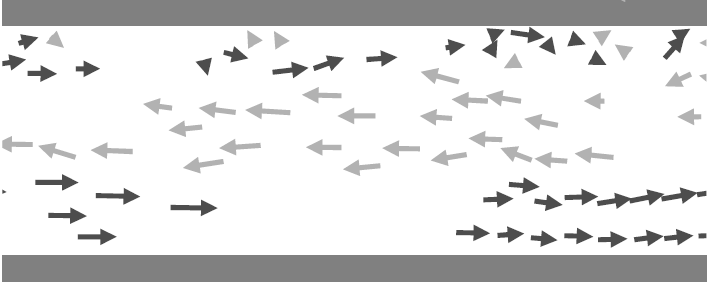
\includegraphics[width=0.7\textwidth]{line.png}
\caption{Formowanie strug, opracowanie \cite{HeBuAjTw}}
\end{figure}

\section{Unikanie Kolizji}
\label{sec:kolizje}

Podczas każdej zmiany położenia podczas symulacji należy upewnić się czy po przejściu nie dojdzie do kolizji z innymi uczestnikami ruchu czy przeszkodami. W przypadku kolizji należy sprawdzić jej typ~i dostosować do niej zachowanie jednostki. Do kolizji może dość w przypadku, kiedy dwoje pieszych~w następnym kroku mają przejść na to samo miejsce lub kiedy zamieniają się miejscami. Każda~z kolizji wymaga podjęcia innych kroków, aby jej uniknąć. Po uniknięciu kolizji pieszy powinien powrócić do swojej pierwotnej ścieżki ruchu. Każdy z pieszych ma także pewien priorytet zależny od takich cech jak niepełnosprawność itp.

Zgodnie z pracą Charif Foudil \cite{Collision} możemy wyróżnić trzy typy kolizji:

\subsection{Kolizja czołowa}

Występuje w przypadku, kiedy dwoje pieszych idzie prosto na siebie. Na samym początku należy określić, czy piesi kolidują ze sobą po lewej czy po prawej stronie (rzadko zdarza się ruch dokładnie na wprost siebie). Piesi preferują takie uniknięcie kolizji, jakie pozwoli im na jak najmniejsze odchylenie od ich wyznaczonej wcześniej trasy. Możemy wyróżnić trzy możliwości uniknięcia takiej kolizji:

\begin{itemize}
\item zmianę kierunku ruchu
\item zmianę prędkości
\item zmianę zarówno kierunku, jak i prędkości
\end{itemize}

Jeśli żaden ze sposobów nie zadziała, pieszy zatrzyma się, przepuszczając drugiego uczestnika ruchu, a następnie ruszy wyznaczoną wcześniej trasą.


\begin{figure}
\centering
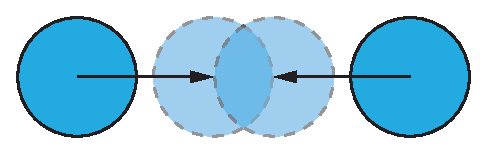
\includegraphics[width=0.4\textwidth]{kolizjaczolowa.eps}
\caption{Schemat kolizji czołowej, opracowanie własne}
\end{figure}

\subsection{Kolizja boczna}

Kolizja, której rozwiązanie jest podobne jak dla \textit{kolizji czołowej}.

\begin{figure}
\centering
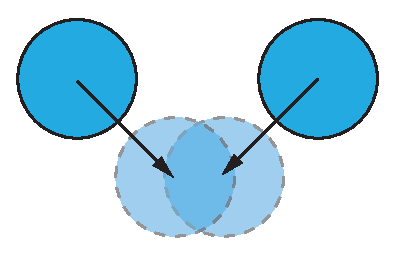
\includegraphics[width=0.4\textwidth]{kolizjaboczna.eps}
\caption{Schemat kolizji czołowej, opracowanie własne}
\end{figure}

\subsection{Kolizja tylna}

Ma miejsc, gdy pieszy porusza się z większą prędkością niż inny uczestnik ruchu pokonujący przed nim tę samą drogę. W tym przypadku pieszy o większej prędkości może:

\begin{itemize}
\item zwolnić do takiej samej prędkości jak pieszy z przodu i iść za nim
\item przyśpieszyć i wyprzedzić kolidującego pieszego z którejś ze stron
\end{itemize}

\begin{figure}
\centering
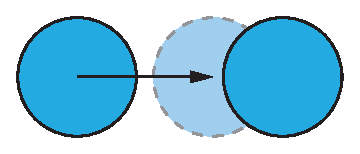
\includegraphics[width=0.4\textwidth]{kolizjatylna.eps}
\caption{Schemat kolizji czołowej, opracowanie własne}
\end{figure}

\chapter{Schematy działania systemu}
\label{cha:schematy}

Pierwszym etapem symulacji było przygotowanie środowiska symulacyjnego. Na zainicjalizowanej dyskretnej siatce \ref{figure:siatka}, zostali wygenerowani piesi oraz przeszkody. W symulacji wykorzystano śmioelementowe sąsiedztwo Moore'a \ref{figure:siatka}.

[Do dokończenia po zaimplementowaniu całości]
\begin{figure}
\label{figure:siatka}
\centering
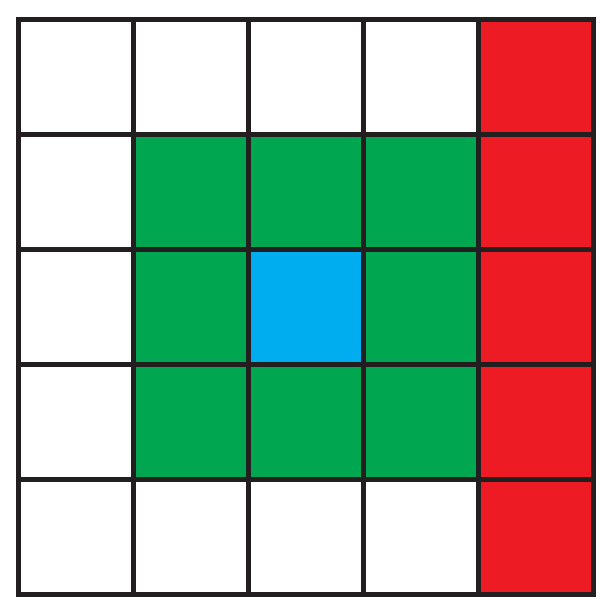
\includegraphics[width=0.4\textwidth]{sasiedztwo.eps}
\caption{Schemat siatki używanej w projekcie. Kolorem niebieskim oznaczono pieszego, zielonym jego sąsiedztwo Moore'a, czerwonym przykładowa przeszkoda}
\end{figure}

Symulacja została zaimplementowana przy użyciu języka Java w wersji 8 we wsparciu biblioteki graficznej Jwjgl.

\section{Przyjęte parametry}
[Do dokończenia po zaimplementowaniu całości]

\chapter{Testy}
\label{cha:testy}

Testy symulacji

\chapter{Podsumowanie}
\label{cha:podsumowanie}

\section{Potencjalne kierunki dalszych prac}
Temat symulacji ruchu pieszych jest bardzo rozległy. Obecne modyfikacje samego SFM pozwalają na implementację różnych zachowań pieszych. Model mógłby zostać wzbogacony o~zachowanie pieszych pod wpływam paniki, zagrożenia (np. związanego z pożarem) lub ruchem innych obiektów (np. samochodów). W modelu możnaby również bardziej zróżnicować pojedynczych agentów, jako że w świecie realnym mamy do czynienia z ludźmi starszymi, którzy poruszają się z~niższą prędkością, dziećmi czy osobami niepełnosprawnymi. Symulacja mogłaby zostać zaimplementowana przy użyciu wielu wątków. Pozwoliłoby to na pokazanie większej ilości detali i~częstosze wyszukiwanie ścieżki ruchu pieszego. Ponadto dla lepszej wizualizacji graficznej model mógłby zostać wzbogacony o~trzeci wymiar. Ciekawym wydaje się również implementacja liderów, którzy istotnie wpływają na zachowanie pieszych w~szczególności w~sytuacjach kryzysowych takich jak ewakuacja, tak jak zaproponowano w pracy (Guided Crowd Dynamics via Modified Social Force Model\cite{GuideCrowdDynViaModifiedSocialForceModel}). Zmodyfikowane modele Social Force pozwalają także na obliczanie ewentualnej ilości ofiar lub osób zranionych, co ma znaczenie w przypadku symulacji ewakuacji. 
Ciekawym wydaje się także zastosowanie logiki rozmytej \cite{modelingFuzzyLogic}.
Temat symulacji jest bardzo rozbudowany, może on zdaniem autora być kierunkiem badań niejednej pracy. 

\section{Wnioski}
\label{sec:wnioski}

Celem niniejszej pracy inżynierskiej była symulacja dynamiki ruchu pieszych. Po porównaniu istniejących modeli wybrany został Model Social Force ze względu na swoje możliwości oraz zastosowanie do problemu postawionego w pracy. Z~sukcesem zaimplementowany został sam model, algorytm wyszukiwania najkrótszej ścieżki, moduł unikania kolizji oraz symulacja graficzna.\\
%----------
Symulacja pozwala na modyfikowanie wielu parametrów takich jak ilość pieszych, rodzaje map, zakresy prędkości czy parametry samego SFM. Dzięki takim możliwościom można otrzymać bardzo ciekawe rezultaty i dogłębnie zbadać dynamikę ruchu pieszych.\\
%---------
Poprzez wielokrotne testy oraz odpowiedni dobór parametrów udało się uzyskać rezultaty odpowiadające rzeczywistości czego potwierdzeniem są przedstawione wykresy oraz ich zgodność z innymi symulacjami \cite{GuideCrowdDynViaModifiedSocialForceModel} i \cite{SocialForceSuwala}

Symulacja nie jest wolna od wad. Czasami zdarzają się zakleszczenia oraz występuje problem wydajnościowy przy większej ilości pieszych (powyżej 90), co uniemożliwia płynne wyświetlanie symulacji. W przypadku większej ilości pieszych występuje także problem z oscylacjami, jednakże jest to znany problem SFM \cite{oscillations}.

Stworzona symulacja może być świetną podstawą do dalszego rozwoju prac. Zdaniem autora aspektami wartymi szczególnie wartymi rozwinięcia jest implementacja różnych sytuacji takich jak ewakuacja pod wpływem pożaru lub innego zagrożenia oraz dalszy rozwój modelu do unikania kolizji pomiędzy pieszymi.

\section{Napotkane problemy}

Istnieje wiele publikacji poświęconych tematyce ruchu pieszych, jednakże większość z nich nie porusza całości problemu. Ciężko jest doszukać się kompleksowego wytłumaczenia wszystkich zjawisk, takich jak formowanie strug czy unikanie kolizji, w obrębie jednego zaproponowanego modelu.

W trakcie tworzenia pracy autor napotkał następujące problemy:

\begin{itemize}
\item wydajność algorytmu A* do wyznaczania optymalnych ścieżek przejścia. Implementacja samego algorytmu nie należy do najbardziej skomplikowanych. Ścieżki zostały łatwo wyznaczone, jednak problem pojawił się przy testach dla większej ilości agentów. Poprzez reprezentację tablicową dwóch zbiorów \textit{open set} oraz \textit{close set}, potrzebnych do działania algorytmu, czas wyszukiwania ścieżki na mapie z ilością węzłów ok. $480000$ wynosił ok. $10 sek$. Jest to czas wysoce odbiegający od potrzeb symulacji. Poprzez reprezentację zbiorów jako stos, czas ten skrócił się do ok. $100-200 ms$ dla takiej samej ilości węzłów. Czas wyszukiwania zależny jest w szczególności od ilości punków węzłowych, ale także od odległości między punktem początkowym i końcowym oraz ilości przeszkód.

\item w praktyce wszystkie publikacje dotyczące tematyki symulacji skupiają się w dużej mierze na opisie konkretnego modelu, nie dotykając przy tym kwestii jego praktycznego zastosowania. Dlatego jednym z największych problemów było zastosowanie wybranego modelu do symulacji.
\end{itemize}


% itd.
% \appendix
% \begin{titlepage}\centering
\vspace*{\fill}
\LARGE Dodatki
\vspace*{\fill}
\end{titlepage}

\begin{samepage}

\chapter{A. Zbiorcze porównanie testów}
\label{cha:dodatekA}

\begin{figure}
\label{figure:siatka}
\centering
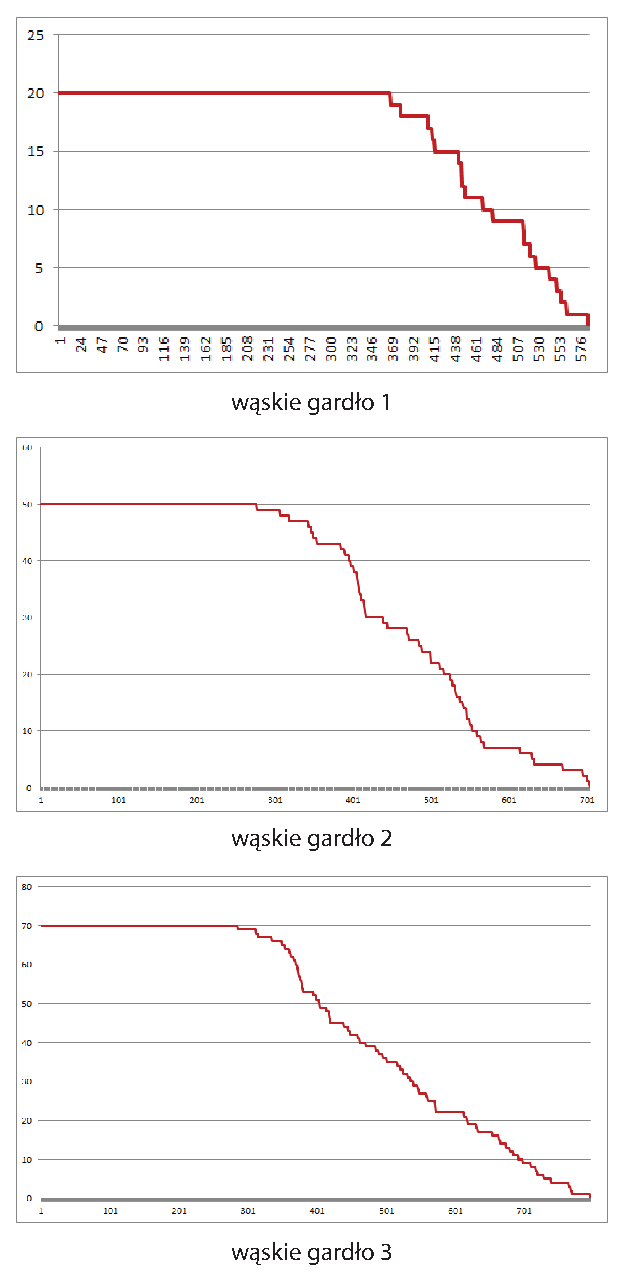
\includegraphics[width=0.4\textwidth]{iloscpieszychwaskie.eps}
\caption{Liczba pieszych w czasie - wąskie gardło}
\end{figure}
\end{samepage}

\begin{figure}
\label{figure:siatka}
\centering
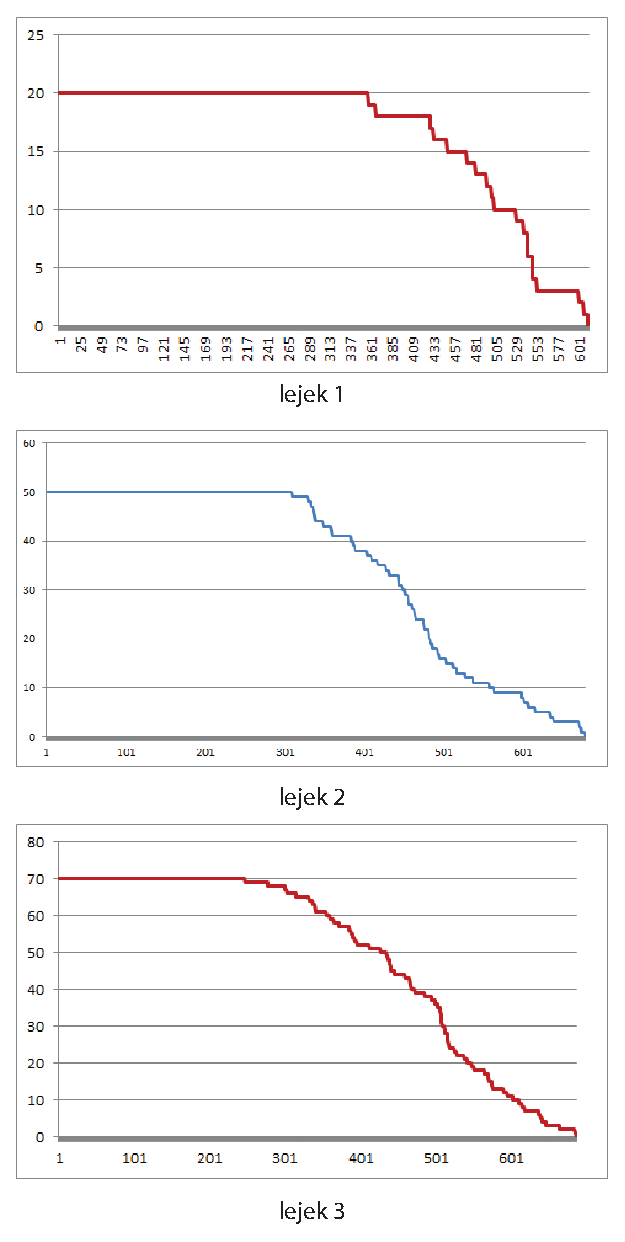
\includegraphics[width=0.5\textwidth]{iloscpieszychlejek.eps}
\caption{Liczba pieszych w czasie - lejek}
\end{figure}

\begin{figure}
\label{figure:siatka}
\centering
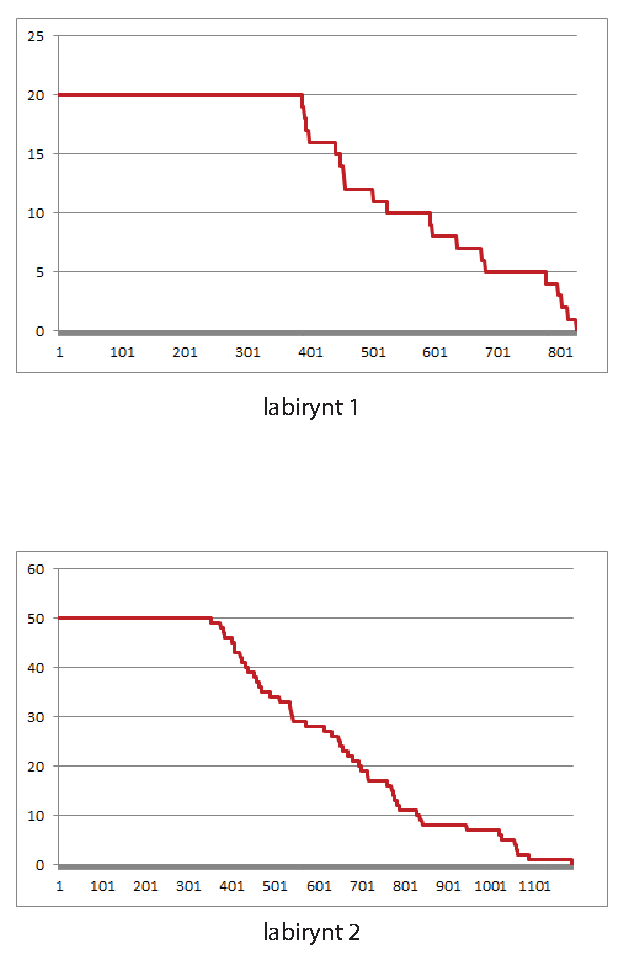
\includegraphics[width=0.5\textwidth]{iloscpieszychlabirynt.eps}
\caption{Liczba pieszych w czasie - labirynt}
\end{figure}

% \include{dodatekB}
% itd.

\printbibliography

\end{document}
